\documentclass[simplex.tex]{subfiles}
% DO NOT INCLUDE PREAMBLES/PACKAGES HERE!!
% packages are inherited from preamble.tex; you can compile this on its own
\begin{document}
\subsection[Randomer Forest]{Randomer Forest (RerF)}

Most recently, we have begun investigating the theoretical behavior of RerF. Mathematical analysis of the RF and RerF procedures is difficult. Therefore, we have started with simplified procedures. The main simplifications we have made are that trees only have a depth of one (also known as decision stumps), and that each tree is trained on the full training set rather than a bootstrap sample. In the figure, we surprisingly see that RerF outperforms RF across a variety of settings (see caption for more details).

\begin{figure}[h!]
\begin{cframed}
\centering
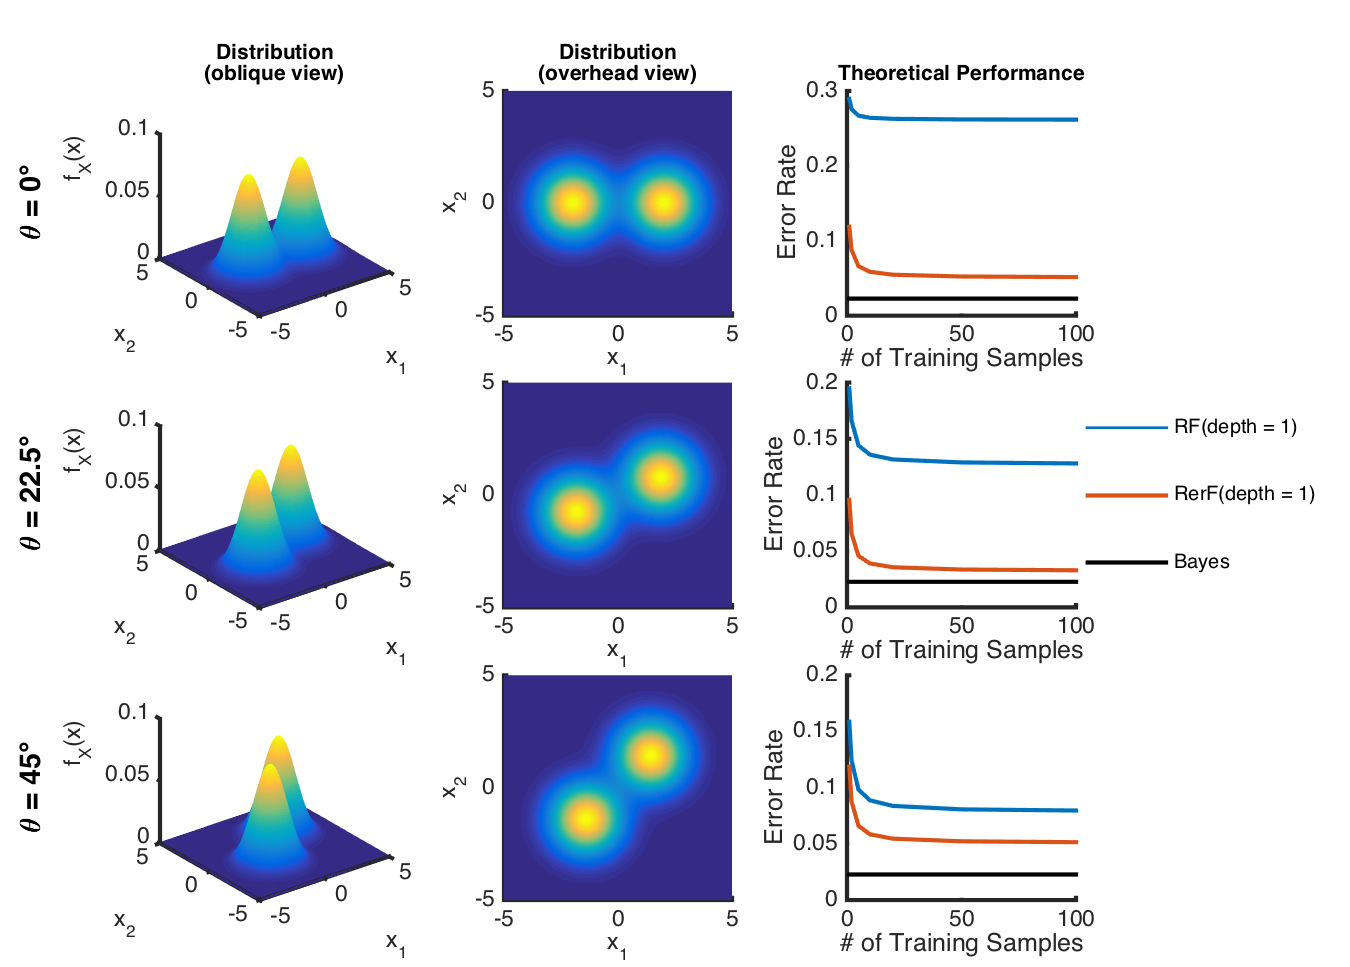
\includegraphics[height=0.4\textheight]{../../figs/RerF.png}
\caption{
Theoretical performances of simplified RF and RerF models on a simple two-dimensional binary classification problem. In the top row, the two classes are distributed according to normal distributions having means that differ only in the first dimension and both having identity covariances. These distributions are shown in the left and middle panels. The right-most panel shows the theoretical error  rate as a function of the number of training samples for RF and RerF. The Bayes optimal error rate is also shown for reference. The middle and bottom rows are the same as the top row, except the distributions have been rotated by 22.5° and 45° respectively. In all three cases, the RerF classifier outperforms RF for all training set sizes.
}
\label{fig:RerF}
\end{cframed}
\end{figure}

\end{document}
